\documentclass[dvipdfmx,autodetect-engine,titlepage]{jsarticle}
\usepackage[dvipdfm]{graphicx}
\usepackage{ascmac}
\usepackage{fancybox}
\usepackage{listings}
\usepackage{plistings}
\usepackage{itembkbx}
\usepackage{amsmath}
\usepackage{svg}
\usepackage{url}
\usepackage{graphics}
\usepackage{listings,jvlisting}

\textheight=23cm
\renewcommand{\figurename}{図}
\renewcommand{\tablename}{表}
\newenvironment{code}
{\vspace{0.5zw}\VerbatimEnvironment  
\begin{screen} 
\baselineskip=1.0\normalbaselineskip
 \begin{Verbatim}}
{\end{Verbatim}
\baselineskip=\normalbaselineskip
 \end{screen}\vspace{0.5zw}} 

\title{情報理工学部 SNコース 2回\\
オブジェクト指向論\\
レポート課題}
\author{2600200443-6\\Yamashita Kyohei\\山下 恭平}
\date{Jan 17 2021}

\begin{document}

\maketitle

\section{オブジェクト指向技術がソフトウェア開発の生産性に対して,どのように役立つのか}
オブジェクト指向技術がソフトウェアの開発の生産性に対して、どのよう役立っているか、これを
知るためにはまず、オブジェクト指向技術の特徴について述べる必要がある。オブジェクト指向とは
何か、Wikipediaには以下のように記されている。
\begin{quote}
  オブジェクト指向プログラミングとは「オブジェクト」という概念に基づいた
  プログラミングパラダイムの一つである。[1]
\end{quote}
プログラムをオブジェクト、物として扱うことで非常に様々な特徴が出現する、その
特徴の一つが、大人数での作業を可能とすることだ。私自身も去年友達二人でSwift言語
を用いてアプリケーションを開発したが、アプリのそれぞれのページに対して各々がコード
を書いていくことが可能なのである。例えば、設定画面は私が作り、ゲーム画面はもう一人
が作る、といったことが可能になるのである。これはオブジェクト指向プログラミングの
大きな強みと言えるだろう。さらに、移す必要のあるデータなどは除いて、プログラム内では
自身が好きなように変数などを使用することができる。これは、それぞれのプログラムが
オブジェクトとして独立しており、後からそれらを組み合わせることで、一つのアプリ
ケーションが出来上がるからである。この具体例から見えるように、オブジェクト指向技術
を用いれば大人数での分担作業が容易になるので、生産性は大きく向上することがわかる。
さらに、アプリケーション開発において新機能を付け足すことも容易に行うことができる、
新機能を追加するということは、新しくオブジェクトを付け足すということであるので、
今まで制作してきた既存のプログラムを改変することなく、付け足す部分だけをプログラム
してやれば、新しく機能を追加することが可能なのである。これは、現代のゲーム
などにおいてよく見られることで、新しいキャラクターが時間と共にどんどん追加されていくのは
オブジェクト指向技術を用いているからと言えるだろう。このように、オブジェクト指向
技術を用いればユーザ、開発者ともに利点があることがわかった、オブジェクト指向技術
を用いると、生産性を上げることができ、ユーザの満足度へとつながるので、結果より良いサービスへ
と繋がっていくと考えられる。

\section{オープン・クローズドの原則}
まず初めに、オープン・クローズドの原則とはWikipediaに以下のように示されている。
\begin{quote}
  ソフトウェア要素(クラス、モジュール、関数など)は、拡張に対しては開いており、
  修正に対しては閉じているべきである。[2]
\end{quote}
これは一つのソフトウェアに対して、ソースコードを変更せずにソフトウェアの動作、
振る舞いを変更可能とするための原則である。言い換えれば、新しい要素を追加するとき
既存のコードは一切変更せず、新しく追加するコードのみを書き足せば良いということである。
この既存のコードに一切の変更を加える必要のないことを「修正に対して閉鎖している」と
表現し、新しくコードを書き足せば良いことを「拡張に対して開いている」と表現する。では
実際にの例を見ていく。\\
クレジットカード決済サービスを考える。また、クレジットカード会社ごとに手続き
が異なるとする。このとき、クラス「クレジットカード」を作り、そのメソッド内で
会社ごとに手続きを分岐したとする。こうした場合、新たなクレジットカード会社が必要
となったとき、既に存在するクラスのメソッドを書き換える必要が出てくる、よって
オープン・クローズドの原則を満たしていないことがわかる。図1はその様子を示した
クラス図である。

\begin{figure}[h]
  \centering
  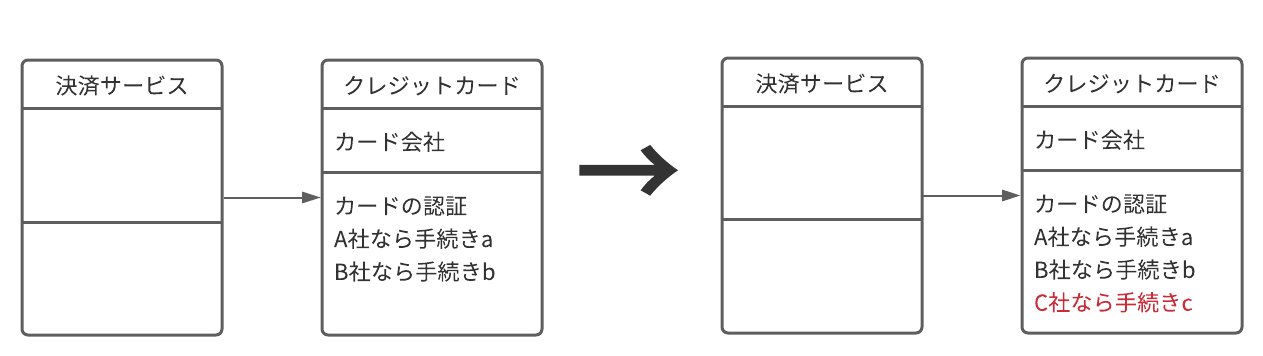
\includegraphics[scale=1]{pic1.png}
  \caption{満たさないクラス図}
\end{figure}

では、オープン・クローズドの原則を満たすにはどのようにすればよいか、それを示したのが
図2である。クレジットカードをインタフェースとし、それぞれのクレジットカード会社クラスに
継承させ、それぞれのクラス内で決済手続きを記述する、そうすることで、新たなカード会社
が増えた時も同様に、インタフェースを継承し手続きを記述するだけで追加することができる。
この時、既存のコードを一切書き換えることなく、新たなカード会社を追加できているので、
これは、オープン・クローズドの原則を満たしていることがわかる。

\begin{figure}[h]
  \centering
  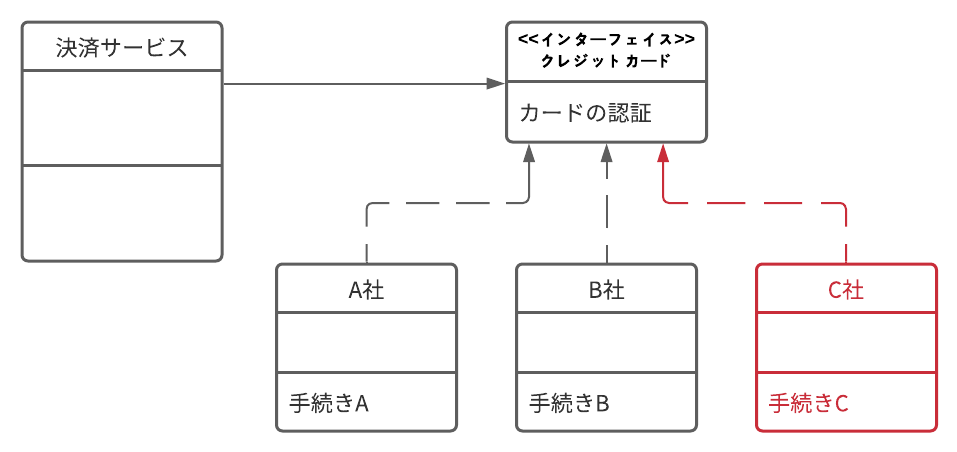
\includegraphics[scale=1]{pic2.png}
  \caption{満たすクラス図}
\end{figure}


\section{図書貸出システムの分析}
このシステムは、会員、貸出・返却、図書、本、雑誌の5つのクラスで構成することが
できる。それぞれのクラスの関係性を示すクラス図を図3に示す。

\begin{figure}[h]
  \centering
  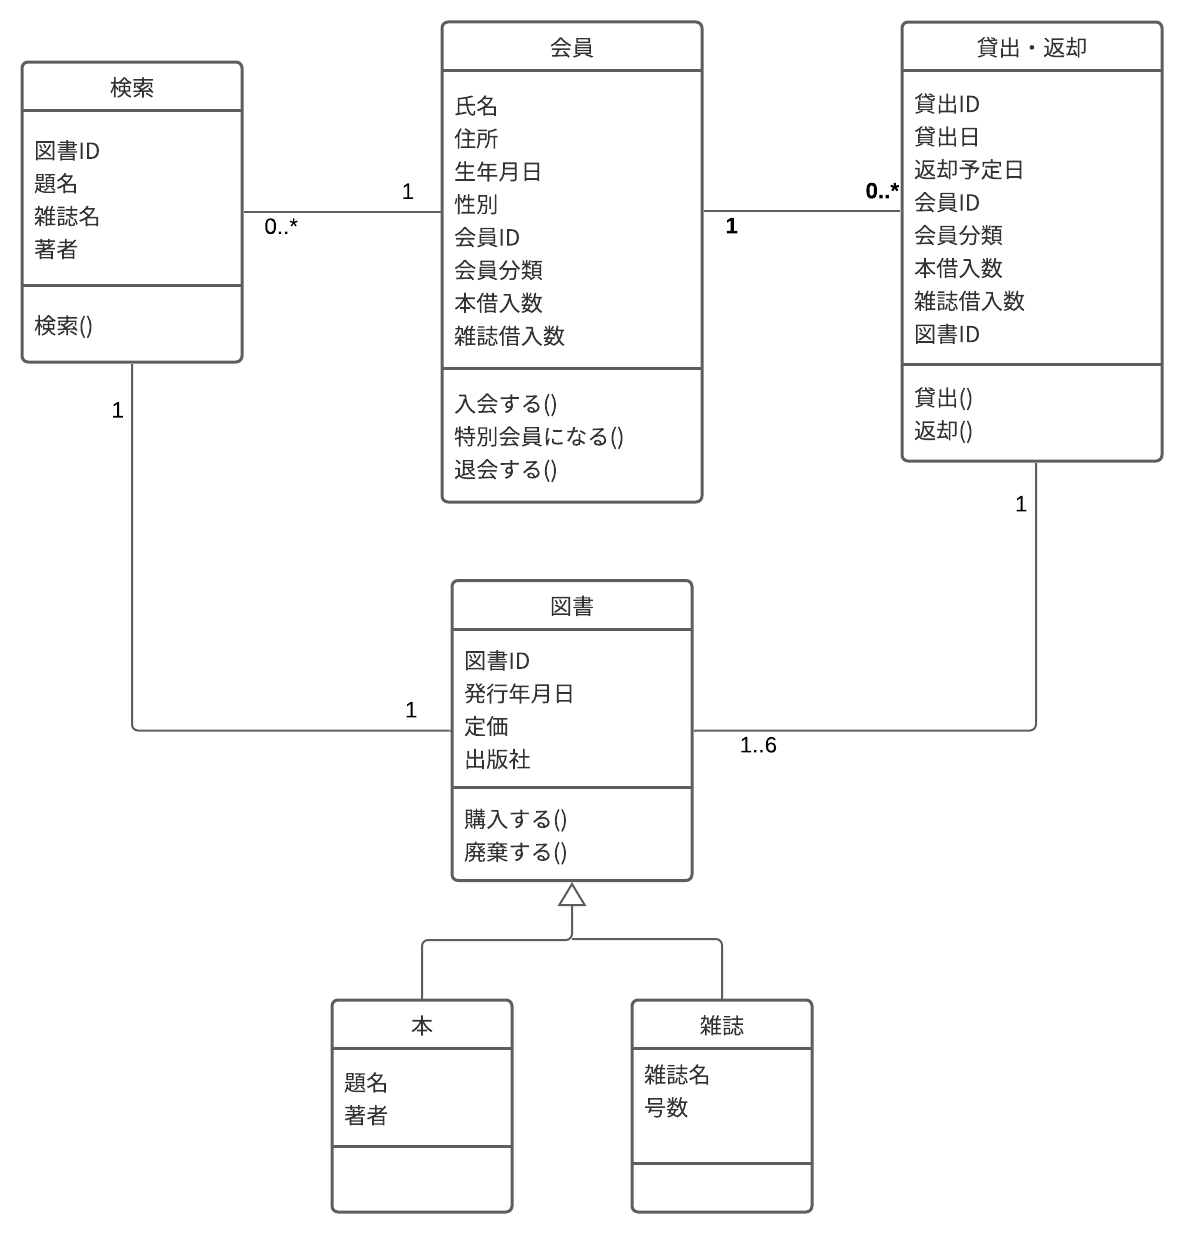
\includegraphics[scale=0.7]{pic3.png}
  \caption{クラス図}
\end{figure}

今回の要求定義では会員の種類は2種類あると読み取れたので、勝手であるが今後会員の
種類は増えないものとして扱った。そうすることで、クラス「通常会員」と「特別会員」
を作らずに、クラス「会員」内の属性として、会員の種類を設けた。クラス「貸出・返却」
では、「会員」インスタンスと関連を持っているので、会員の種類ごとに貸出可能かどうかを
、クラスのメソッドで分岐させている。クラス「図書」ではクラス「本」「雑誌」を図書
から継承させ、新しい本や雑誌が入った時も、少ない情報で新たに登録可能とした。
クラス「検索」では、クラス「図書」と関連を持たせ、入力された文字列と比較することで
検索機能を実現させている。

以下の図4は貸出時のオブジェクトとの相互作用を時系列に示した図である。初めに
クラス「会員」はクラス「貸出・返却」に自信の会員IDを送り、「貸出・返却」は
貸出数が上限に達していないかを確認後、貸出許可を出す。その後会員は借りたい本のID
を入力し、「貸出・返却」はクラス「図書」へ問い合わせを行う。今回の要求定義では本は
複数存在するので、貸出できないことは無視できる。最後に本を借りれたクラス「会員」は
自信の貸出数を更新し終了する。


\begin{figure}[h]
  \centering
  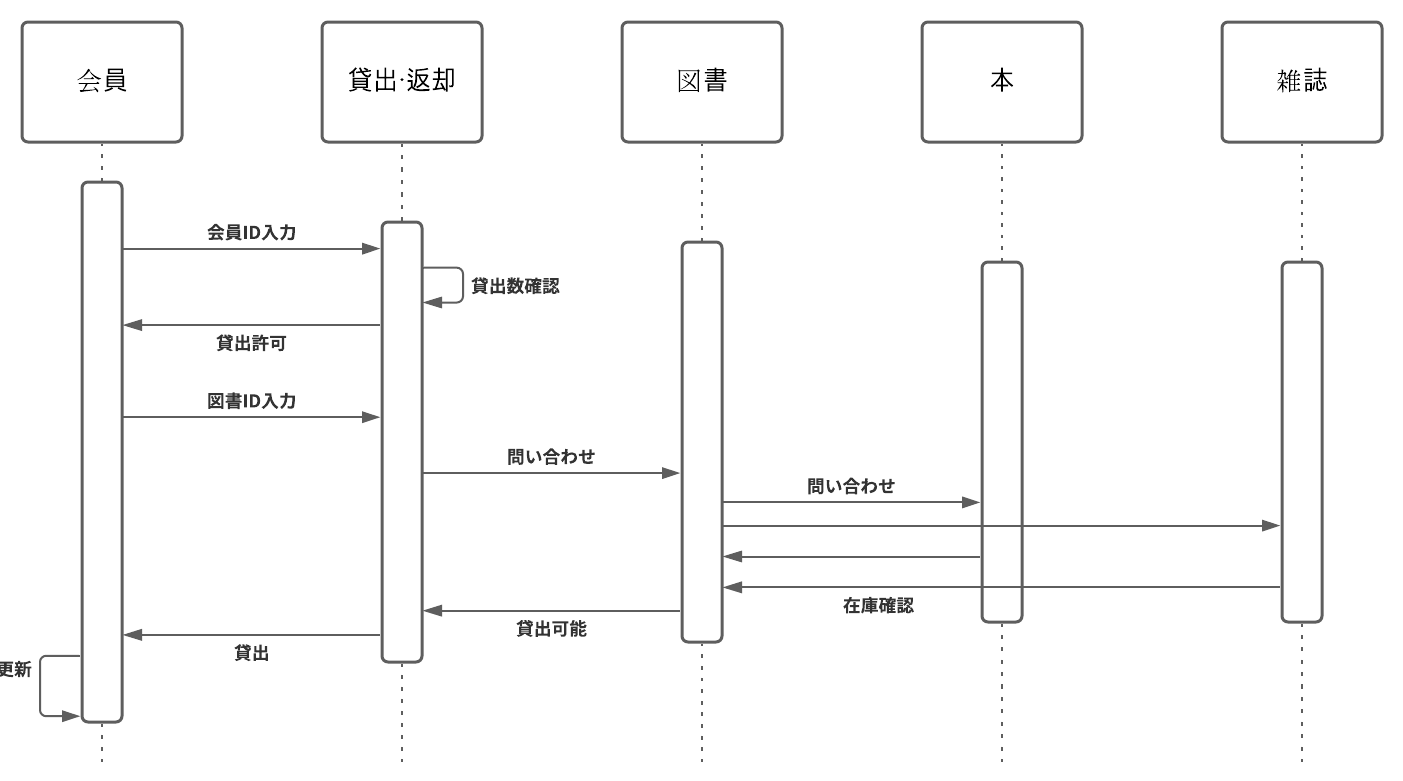
\includegraphics[scale=1]{pic4.png}
  \caption{貸出時のシーケンス図}
\end{figure}

以下の図5はクラス「会員」が取り得る状態を示した、状態機械図である。初めに、検索中は
会員であればいつでも利用できる。次に貸出・返却だが、これは会員の現在借りている本の
冊数によって状態が異なってくる。まず、貸出可能状態だが、これは図書、雑誌どちらか一方
の貸出数が上限に達していなければこの状態に遷移する。この状態では、貸出、返却どちらの
メソッドも可能である。次に貸出不可能状態は、本、雑誌それぞれの貸出上限冊数に到達
している時この状態に遷移する、この状態では返却メソッドしか行うことができず、返却
を行うと、もれなく、貸出可能状態へと遷移する。貸出可能状態で貸出を行なった時は、再び
貸出可能状態へ遷移するか、貸出不可能状態へと遷移する。

\begin{figure}[h]
  \centering
  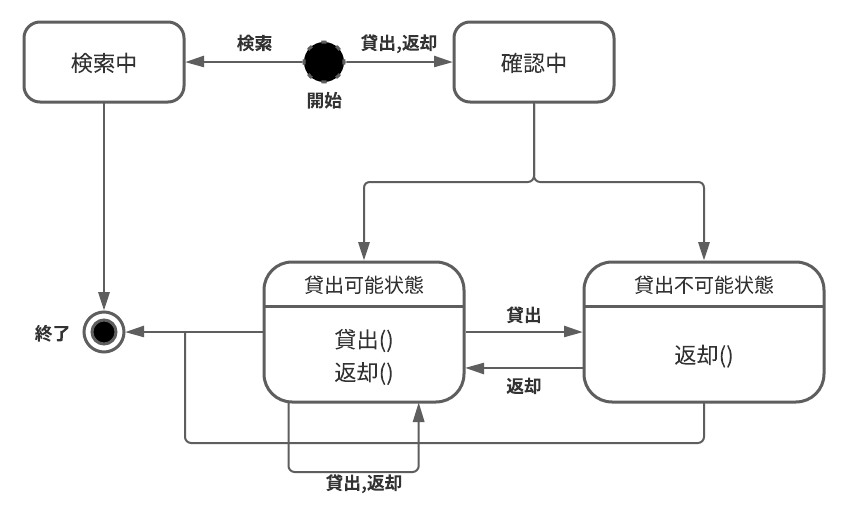
\includegraphics[scale=1]{pic5.png}
  \caption{状態機械図}
\end{figure}

\section{参考文献}

[1]Wikipedia,オブジェクト指向プログラミング\\
\url{https://ja.wikipedia.org/wiki/オブジェクト指向プログラミング}\\

[2]Wikipedia,開放/閉鎖原則\\
\url{https://ja.wikipedia.org/wiki/解放/閉鎖原則}



\end{document}

